\chapter{Common Kernel Functions}
\lhead{Common Kernel Functions}
\label{Appendix:CommonKernelFunctions}

	While the squared exponential kernel suffices for most Gaussian process based inference, in general the choice of kernel covariance allows one to better adapt to the data at hand in order to achieve better predictive capabilities.
	
	This section extends the discussion in Section \ref{Background:GaussianProcesses:KernelFunctions} and covers the widely used \matern class kernels and the non-stationary Paciorek kernel. Again, the following discussion will only cover the minimal background for the structure and significance of kernel functions, as treatments of kernel functions can easily become very detailed and rigorous in topics such as differentiability effects or eigenfunction decomposition.
	
	\section{Other Stationary Kernels}
	\label{Appendix:CommonKernelFunctions:Stationary}
	
		Continuing with the formulation in Section \ref{Background:GaussianProcesses:KernelFunctions}, the \matern class of kernel functions are given by \eqref{Equation:MaternKernel}.
		
		\begin{equation}
			\left.
				\begin{aligned}
					k_{\mathrm{\maternmath}}(\bvec{x}, \bvec{x}') =& \; \sigma_{f}^{2} \frac{2^{1 - \nu}}{\Gamma(\nu)} \Big( \sqrt{2 \nu} a \Big)^{\nu} K_{\nu}\Big( \sqrt{2 \nu} a \Big) \\
					a^{2} :=& \; (\bvec{x} - \bvec{x}')^{T} \Sigma^{-1} (\bvec{x} - \bvec{x}')
				\end{aligned}
			\qquad \right.
		\label{Equation:MaternKernel}
		\end{equation}
					
		Here, $\Gamma$ and $K_{\nu}$ are the Gamma function and modified Bessel function respectively, while $\nu$ is a positive hyperparameter that determines the differentiability property of the \matern class kernel. The GP model with \matern class kernel is $d$-times mean square differentiable if and only if $\nu > d$ \citep{GaussianProcessForMachineLearning}. In the limit of $\nu \rightarrow \infty$ for infinite differentiability, the \matern kernel becomes the squared exponential kernel \eqref{Equation:SquaredExponentialKernel}. While the general \matern class kernel seem complicated due to the Gamma function and modified Bessel function, its form become simple for $\nu = p + \frac{1}{2}$ where $p$ is a non-negative integer. That is, \matern kernels with $\nu = \frac{1}{2}, \frac{3}{2}, \frac{5}{2}, \frac{7}{2}, \dots$ have simple analytic forms without reference to the modified Bessel function. In fact, for $\nu > \frac{5}{2}$, the degree for which the \matern kernel changes becomes quite unnoticeable for most practical purposes such that it may as well be replaced by the squared exponential kernel with $\nu \rightarrow \infty$. Similarly, while there is a more noticeable effect of changing $\nu$ within the range $\nu \in (0, \frac{5}{2})$, in practice is it is often not worth the expense of implementing the complicated form for a almost unnoticeable improvement in modeling accuracy. Hence, it is replaced with the \matern kernel with $\nu = \frac{1}{2}, \frac{3}{2}, \frac{5}{2}$, whichever is the closest. In this way, in practice only the \matern kernels with $\nu = \frac{1}{2}, \frac{3}{2}, \frac{5}{2}$ are employed, and they are respectively termed the \matern 1/2 kernel, \matern 3/2 kernel, and \matern 5/2 kernel - in the order of increasing differentiability. These kernels have the forms listed below \eqref{Equation:PracticalMaternKernels}.
		
		\begin{equation}
			\left.
				\begin{aligned}
					k_{\mathrm{\maternmath}, \; \nu = \frac{1}{2}}(\bvec{x}, \bvec{x}') =& \; \sigma_{f}^{2} \exp ( -a ) \\
					k_{\mathrm{\maternmath}, \; \nu = \frac{3}{2}}(\bvec{x}, \bvec{x}') =& \; \sigma_{f}^{2} (1 + \sqrt{3} a) \exp ( -\sqrt{3} a ) \\
					k_{\mathrm{\maternmath}, \; \nu = \frac{5}{2}}(\bvec{x}, \bvec{x}') =& \; \sigma_{f}^{2} \Big(1 + \sqrt{5} a + \frac{5}{3} a^{2}\Big) \exp ( -\sqrt{5} a )  \\
					a^{2} :=& \; (\bvec{x} - \bvec{x}')^{T} \Sigma^{-1} (\bvec{x} - \bvec{x}')
				\end{aligned}
			\qquad \right.
		\label{Equation:PracticalMaternKernels}
		\end{equation}			
		
		Together, the squared exponential kernel and the \matern class kernels provide a flexible set of kernel functions that can model a multitude of phenomena from various fields such as geology, ecology, finance, logistics, control theory, and machine learning.
		
	\section{Non-Stationary Kernels}
	\label{Appendix:CommonKernelFunctions:NonStationary}
	
		Non-stationary kernels introduce flexibility for modeling phenomenons where the inherent length scales varies across feature locations. The limitations with stationary kernels is that the GP will always learn length scales that are as small as it needs to be for modeling the fastest varying phenomenon in the model. While the marginal likelihood inherently balances modeling accuracy and overfitting, when it comes to the choice between modeling a peak in data variation with a risk of overfitting the rest of the data or ignoring that peak, the optimiser will always prefer the former as marginal likelihood gain from successful modeling is higher than loss from overfitting. Because learning stage is done through optimising the marginal likelihood (see Section \ref{Background:GaussianProcesses:Regression:HyperparameterLearning}), this forces the length scale to be smaller than it needs at slower varying places.

		Figure \ref{Figure:GaussianProcessLengthScale} illustrates the non-stationary Gaussian process for a terrain modeling application, where flat regions have high length scales (slow varying) while rough regions have low length scales (fast varying). Note that this does not imply that it is only relevant for GP regression problems - the latent functions used in GP classification is itself a GP regression problem for which length scale interpretation is almost identical to that shown in Figure \ref{Figure:GaussianProcessLengthScale}.
		
		\begin{figure}[!htbp]
			\centering
				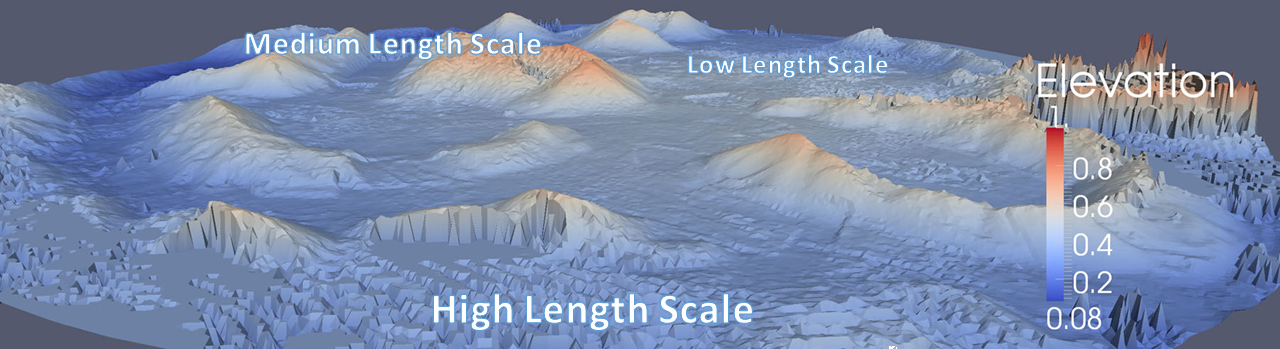
\includegraphics[width=\textwidth]{Figures/gaussianprocesslengthscale.png}
			\caption{Non-stationary Gaussian process for seafloor terrain modeling Adapted from \cite{ROB:ROB21403}}
			\label{Figure:GaussianProcessLengthScale}
		\end{figure}
		
		The non-stationary kernel function employed in this thesis is the Paciorek non-stationary covariance kernel function \eqref{Equation:NonStationaryKernel} \citep{AdaptiveNonStationaryKernel}.
		
		\begin{equation}
			k(\bvec{x}_{i}, \bvec{x}_{j}) = \sigma_{f}^{2} |\Sigma_{i}|^{\frac{1}{4}} |\Sigma_{j}|^{\frac{1}{4}} \Bigg|\frac{\Sigma_{i} + \Sigma_{j}}{2}\Bigg|^{-\frac{1}{2}} \exp\Bigg[ -\frac{1}{2} (\bvec{x}_{i} - \bvec{x}_{j}) \Bigg(\frac{\Sigma_{i} + \Sigma_{j}}{2}\Bigg)^{-1} (\bvec{x}_{i} - \bvec{x}_{j}) \Bigg]
		\label{Equation:NonStationaryKernel}
		\end{equation}			
		
		The matrices $\Sigma_{i}$ and $\Sigma_{j}$ are the local length scale matrices at $\bvec{x}_{i}$ and $\bvec{x}_{j}$ respectively, and are interpreted the same way as the stationary case. The only difference is that these length scale matrices only operate locally, and are functions of the input feature vector $\bvec{x}$. In each kernel location, two length scale matrices are queried. Hence, in a kernel matrix of size $n \times m$, maximally $n + m$ unique queries are made if no feature locations overlap.
		
		It is worthwhile to observe that the effective length scale matrix in the exponent is the average of the two length scale matrices, with its effect reduced with increasing distance between the two points of consideration as with all kernels.
		
		Note that the normalisation matrix determinants are chosen such that the kernel function is reduced into the squared exponential stationary kernel when $\Sigma_{i} = \Sigma_{j} = \Sigma$, as derived in \eqref{Equation:NonStationaryKernelToStationaryKernel}. 

		That is, the Paciorek non-stationary kernel reduces to the squared exponential kernel under the stationary limit. In this way, the Paciorek kernel generalises the squared exponential kernel.
				
		\begin{equation}
			\left.
				\begin{aligned}
					k(\bvec{x}_{i}, \bvec{x}_{j}) &= \sigma_{f}^{2} |\Sigma|^{\frac{1}{4}} |\Sigma|^{\frac{1}{4}} \Bigg|\frac{\Sigma + \Sigma}{2}\Bigg|^{-\frac{1}{2}} \exp\Bigg[ -\frac{1}{2} (\bvec{x}_{i} - \bvec{x}_{j}) \Bigg(\frac{\Sigma + \Sigma}{2}\Bigg)^{-1} (\bvec{x}_{i} - \bvec{x}_{j}) \Bigg] \\
					&= \sigma_{f}^{2} |\Sigma|^{\frac{1}{2}} |\Sigma|^{-\frac{1}{2}} \exp\Bigg[ -\frac{1}{2} (\bvec{x}_{i} - \bvec{x}_{j}) (\Sigma)^{-1} (\bvec{x}_{i} - \bvec{x}_{j}) \Bigg] \\
					&= \sigma_{f}^{2} \exp\Bigg[ -\frac{1}{2} (\bvec{x}_{i} - \bvec{x}_{j}) \Sigma^{-1} (\bvec{x}_{i} - \bvec{x}_{j}) \Bigg]
				\end{aligned}
			\qquad \right.
		\label{Equation:NonStationaryKernelToStationaryKernel}
		\end{equation}		